\documentclass[letterpaper]{article}
\usepackage{aaai}
\usepackage{graphicx}
\usepackage{times}
\usepackage{helvet}
\usepackage{courier}

\title{NewsPet}
\author{Michael Fulker, Anthony Hauber \and Tyson Williams \\
COM S 472 : Principles of Artificial Intelligence\\Department of Computer Science\\ Iowa State University, Ames, IA 50011\\
\texttt{\{calculo, thauber, tyson\}@cs.iastate.edu}}
\begin{document}
\nocopyright
\maketitle

\begin{abstract}
For companies that do work updating data based on news stories, many man-hours are wasted by reading irrelevant articles.
We aim to enhance productivity of this work by creating and analyzing NewsPet: an automated news-feed categorizer which utilizes a Naive Bayes text classifier.
\end{abstract}

\section{Introduction}
One of the team members, Michael Fulker, is currently an intern for a company that does management and maintaining of data about companies (relationships between companies, company executives, and other such information).
The idea for this project was inspired by a full-time coworker of Michael, who stated it would be nice to be able to use some sort of AI system to analyze news feeds to and mark items relevant to changes in company relationships and similar information.

As an attempt to create a solution for this problem, we decided to build a web application around a Naive Bayes classifier. Not being limited to Boolean classification (i.e. ``spam'' and ``not spam''), this application allows users to create an arbitrary number of categories, as well as set up an arbitrary number of news feeds to scan. Our system then places news items into these categories according to its current knowledge, and allows the user to submit performance feedback as training (by either manually ``starring'' or recategorizing items).

\pagebreak
\section{Architecture}
The system is designed as follows:

\noindent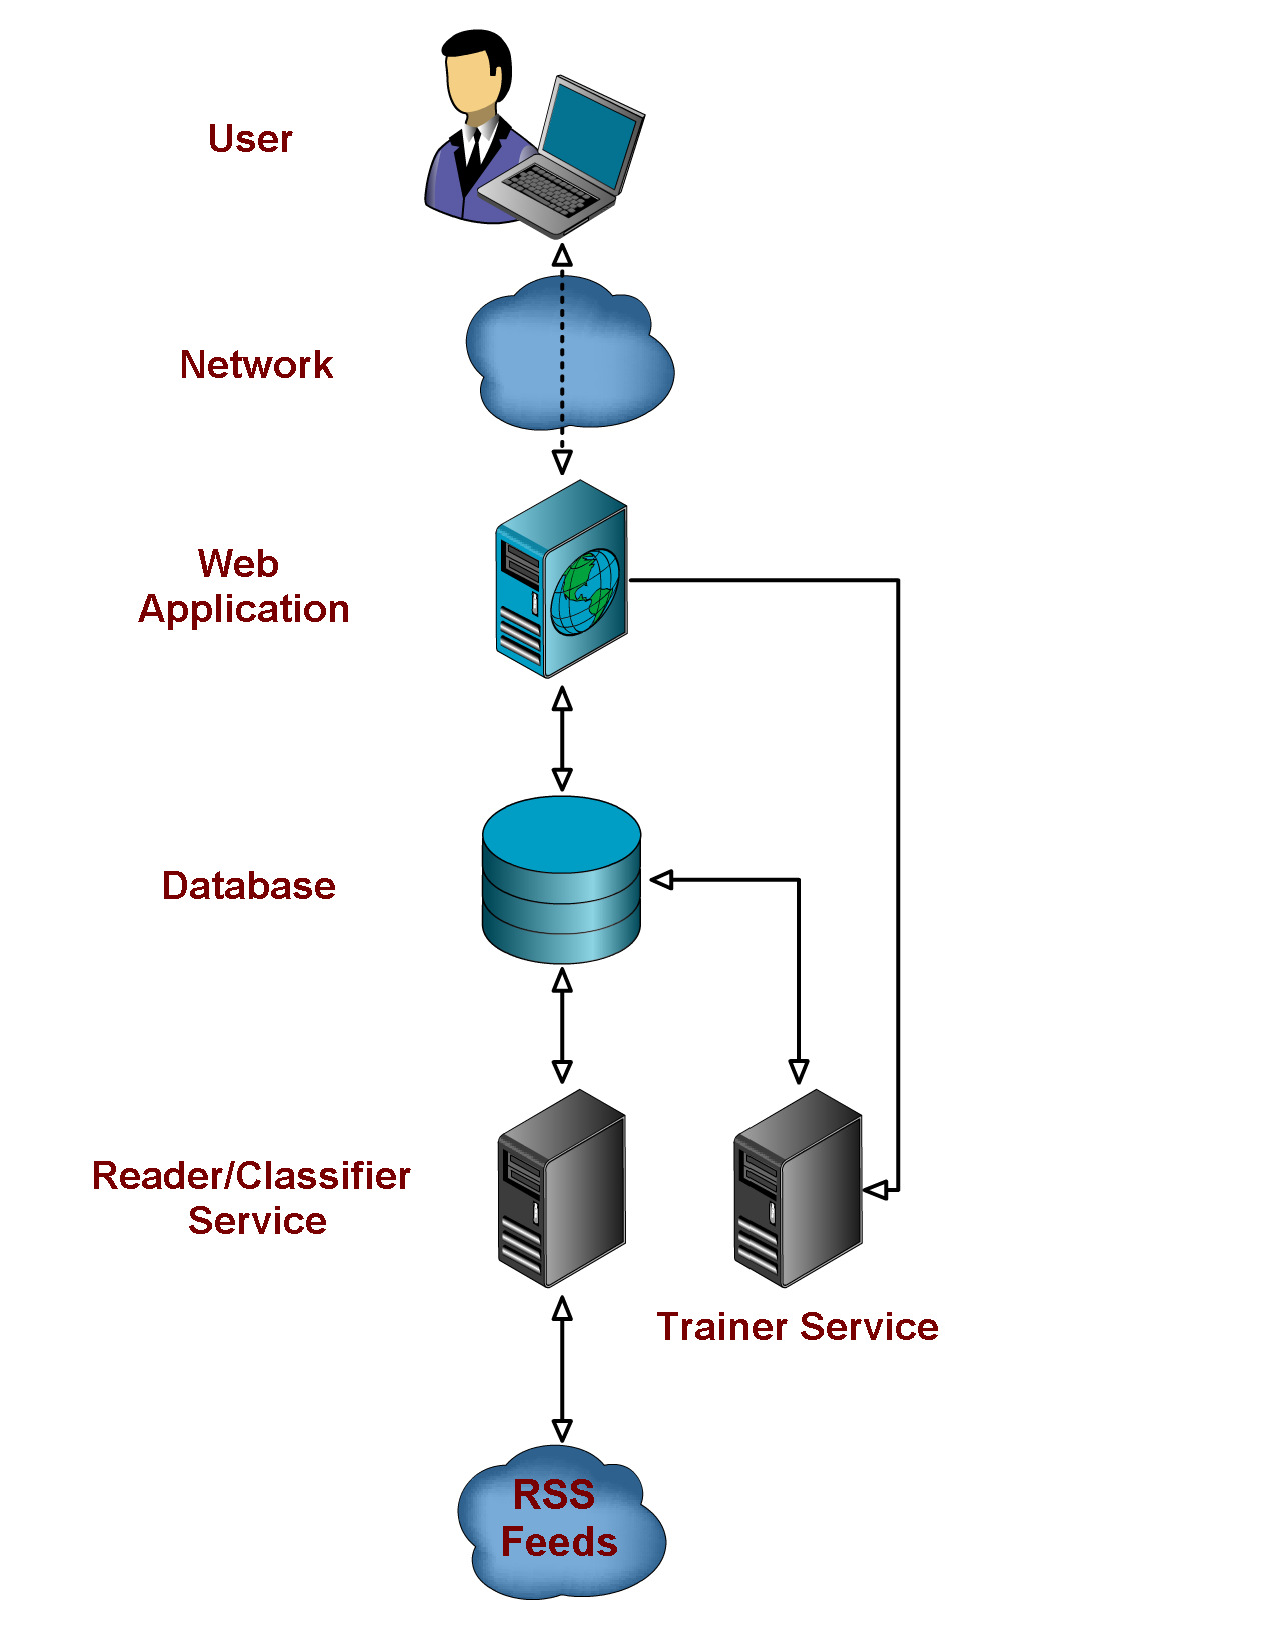
\includegraphics[width=4in]{arch-diagram.pdf}

The web application serves as the user interface, and displays/updates information on the database.
Whenever a user gives input that serves as training data, the appropriate information is put on the database and a signal is sent to the trainer service telling it what to process.

The reader service checks RSS feeds at regular intervals, classifies their news items, and stores them to the database.

The trainer service listens for signals from the web application, and trains/updates database-stored classifier objects according to the indicated training data.

\subsection{Database}
The database is structured as follows (omitting tables automatically set up by the Django framework):

\noindent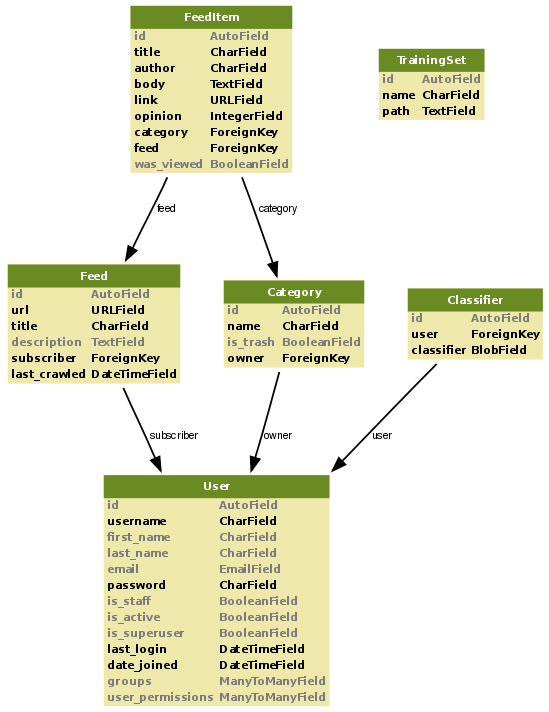
\includegraphics[width=3.5in]{db-diagram-no-transparency.png}

(Arrows indicate a foreign key reference)

A user has multiple feeds, multiple categories, and one classifier object.

A feed item belongs to a single category and a single feed.

A training set consists of a file path on the application server where a text file can be found.

A classifier record stores the serialized form of all objects needed for classifying and training.

\section{Implementation}
\subsection{Web Application Service}
The web application service is responsible for retrieving user input, manage the creation and edition of feeds and categories, displaying feed items, and managing authentication of the users.

\subsubsection{Overview}
The system is split into four modules: Training, Model, View, Controller.  The Controller module is responsible for processing the requests and sending the responses, the Model module persists objects to the database, the View module contains information about the environment that the user will operate in, and the training module alerts the trainer service of new training operations the user has decided on. 

\noindent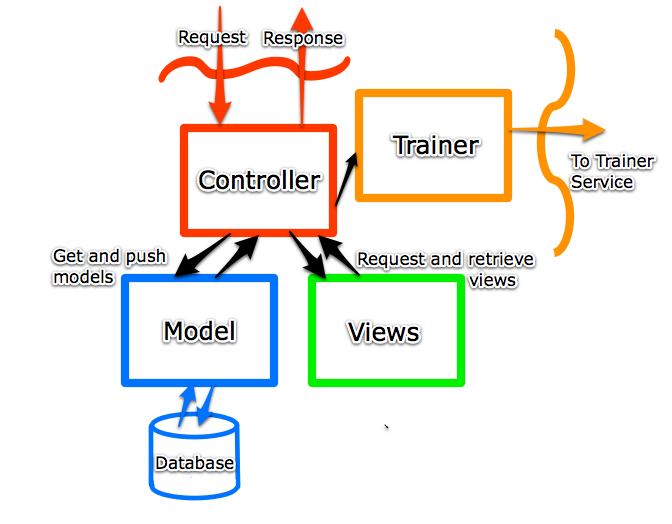
\includegraphics[width=3.5in]{MVC.png}

There are several actions the user is able to do: ``starring'' an item (giving positive feedback), recategorizing an item, creating or editing a category, creating or editing a feed, logging in and out, and viewing feed items . 

The training actions -- starring and moving a feed item, and creating a category -- use the Training module. This module contacts the training service via the Python to Java message queue. To not interrupt the user's experience, a thread is create with a Python2Java socket wrapper that sends a set of predefined messages to the trainer service message queue. 
  
Logging in and out creates and destroys sessions via cookies in the client side browser. This portion of authentication is handled at a controller level. The database only stores hashed versions of the password so they are not readable by us. 

If users add, edit, or delete feeds, the web application access its Model module to edit the database itself.  Feeds have a field which contains the date it has last been crawled.  This is used by the reader service to sort the feeds by priority for reading.  When created feeds are given the date January 1st, 2000, so it will immediately be crawled.  Therefore no direct interaction is needed between the reader service and the web application service.

\subsubsection{Technologies}

The web interface is purely HTTP.  It can be reached by requesting pages from a server.  All of the client-side code (strictly code to enhance user interaction, i.e. slide-down windows and collapsible categories) is written in JavaScript and run in the user's internet browser. The templates for the pages are written to HTML 4.0 standards. To handle requests on the server, we have implemented an Model-View-Controller patter using Django, a Python web-framework.  


\subsection{Trainer Service}
The trainer service checks a message queue (see Message Queue subsection) to get training items, each of which consists of a classifier ID, a desired category ID, and a location to find text (either a training set record, or a feed item record).
Whenever a message or messages are available on the queue, a batch of training items of the same classifier ID are collected, which are put in a runnable job for execution by a threadpool.

If multiple batches have the same classifier ID (for example, if new items are added to the message queue when a thread is in the process of training), the access layer for the classifier/trainer objects ensures subsequent threads ones must wait for the preceding thread to finish.

The actual training is done with \texttt{NaiveBayesTrainer} objects from the Mallet framework \cite{McCallumMALLET}.
Each training thread acquires a trainer object (either deserialized from database, or instantiated for initial training),
passes the training items through a custom filter such that they are converted to objects the Mallet framework is compatible with,
runs these instances through the trainer,
and persists the trainer and classifier back to the database.

A benefit to using this particular framework is that the trainer does not need to know all of the possible categories beforehand. It is possible for a user to add a category and the trainer subsequently receive incremental training items for it, since it detects when new categories are seen and internally modifies its data structures as needed.

\subsection{Reader/Categorizer Service}
The reader service retrieves a list of Feed urls from the database using a certain polling interval. Each time it does this, it creates and starts a series of threadpool jobs to retrieve the RSS data (using the Informa framework \cite{Informa}). When these jobs have all finished, the service creates another series of threadpool jobs, one for each news item. Each of these threads will retrieve the latest classifier for their associated user (deserialized from database), use it to determine the best category, and store their item to the database with the corresponding category ID.

The classifier object is a \texttt{NaiveBayes} classifier from the Mallet framework (trained by the trainer service). The classifier can return a vector of category/probability pairs. The thread doing the classifying will determine the most probable category, and confirm that its probability scaled by the number of categories is at least greater than some value, and categorizes it as trash otherwise. (The rationale for this being that if there are three categories where the most probable category has probability 0.34, and the others have probability 0.33, then this represents a very uncertain classification, and it would be better to put it in the trash as effectively uncategorized.)

\subsection{Message Queue}
\label{MessageQueueSection}
The trainer service uses a custom Message Queue module for receiving user feedback on classification. The feedback from a single user is used for further training of the Naive Bayes classifier. The training requests are sent from the frontend webserver to another server using sockets. We did this to communicate between our frontend python code and backend Java code, but this structure is also useful in that it moves work off of the webserver. The Message Queue is necessary because we wanted to ensure that all user feedback was processed and that it was processed in order.

\subsection{Remark on Classifier Choice}
We wanted to incorporate pre-made libraries in our project where possible, and the classifier was no exception. We considered several different classification frameworks, including Weka and jBNC.

The common way to represent documents when utilizing Naive Bayes is in a feature vector form: each document is represented by an $n$-dimensional vector, given $n$ words in the vocabulary, where the value at a word's index is 1 (or optionally the number of occurrences), and 0 otherwise.

Clearly since most documents don't consist of the entire English language, most of these vectors are very sparse (have mostly zeros).
A major performance issue encountered was that some frameworks stored such a vector in a non-sparse manner, leading to problems with memory usage when training on moderately large data sets.

Another problem encountered was how some frameworks did not seem to be intended for developer use, and were intended to be used only as a standalone program. The problems encountered with these were sparse/nonexistent documentation, non-modular code, and overall difficulty of incorporating into a different project than their own.

We eventually decided on Mallet, due to how it has comparatively reasonable performance and how it lends itself better to developer use. There are still some places where some performance enhancements could be done, for example: each classifier keeps its own hashtable of words to vector-indices, meaning many classifiers being serialized and stored on a database have large amounts of vocabulary information that could be consolidated into a global lookup table. We are ignoring this efficiency problem for now, since the serialized classifiers are currently only 1MB or less in size (which a database can still reasonably handle), and fixing it would require much re-engineering.

\section{Analysis}
Quantitative analysis of the Mallet Framework's Naive Bayes classifier was done using data from Reuters-21578 corpus \cite{Reuters21578} (a collection of pre-categorized news articles made available for research purposes).

Since some of the news articles in this collection are listed under multiple categories, and our model allows one category per news item, we set up our parser to ignore all items that span multiple categories. Out of the 21578 articles, there are 9002 that have singular categories, (this creates a set of 66 possible categories for testing).

We created an analysis program to use a Mallet Naive Bayes classifier in the same manner in which it is used in the main project, train it using a variable portion of the data (randomly selected), and test it using the remaining portion.

We also set up a testing option where a number of categories are artificially grouped together as a ``trash'' category, to simulate typical use of our system. The categories that are grouped together are chosen by the test program randomly at runtime.

For each case of setting the number of non-trash categories to 66, 30, and 5, we ran $16\times 19=304$ trials, (16 trials for each of 19 different training ratios). Results are given below.

\subsection{Results}
Each marker represents the average accuracy of the 16 trials for the specified number of non-trash categories and number of training items.

The error bars signify the maximum and minimum accuracies found over the 16 trials.\\

\noindent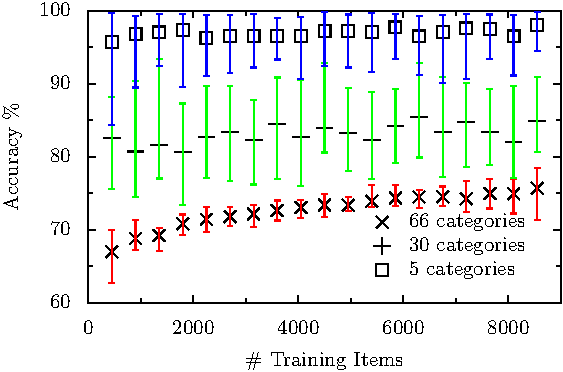
\includegraphics[width=3.35in]{data.pdf}

\subsection{Conclusion}
From the above test results, it is apparent that our initial goal of at least 75\% average accuracy is achieved, provided that the user has a reasonably small number of categories, and/or the classifier has a large enough set of training examples. (To be precise, the classifier had over 75\% average accuracy if over 8550 training items were used in the all-category case, or if over 450 training items were used in the 5-category case.)

\section{Future Work}
We believe that this project has potential beyond this course. It is a novel idea in line with the current trend of online services.

The Mallet framework has preformed wonderfully in our project. However, it does have one major disadvantage. Once it has been trained on a class, it will always remember that class. A standard use case for our program involves the deletion of a category by the user, but the Mallet classifier does not support this action. We have thought about a few ways to solve this. The ineloquent solution is to have a classifier for each category (instead of each user) and use each of them as described in class. That is, ask each classifier for its probability that a given article has that class and return the class with the highest probability. A better solution would be to modify the Mallet source code to allow the deletion of a class. It may be possible to negatively train the Mallet classifiers, but this approach would require a batch training job consisting of all articles previously identified as being in this category.

Overall, we are pleased with the success of our project, and we plan to continue improving upon it in terms of usefulness and scalability.

\bibliography{bibliography}
\bibliographystyle{aaai}
\end{document}
